In diesem Kapitel wird erörtert, wie und aus welchen Elementen, sich das einstehende Softwareprojekt gliedert. Dabei wird jedoch nur die grobe Struktur des Projekt und die für den Anwendungsfall relevanten Aspekte beleuchtet.

Das Projekt ist in \textit{Java} implementiert. Um grafische Benutzeroberflächen zu ermöglichen, wird \textit{JavaFX} eingesetzt. Das Projekt richtet sich nach dem MVC-Modell aus \cite{web:mvc}.

\begin{sloppypar}
Kernaspekt des Projekt ist der Agent. Dieser ist in Form der Klasse \texttt{codyAgent.CoDyAgent} implementiert, die die Klasse \texttt{jade.core.Agent} erweitert. Ein \textit{CoDy-Agent} implementiert, abgesehen von der Wegplanung, die Logik des CoDy Algorithmus. Die Wegplanung ist in Objekten gekapselt, die den verschiedenen Kartentypen des CoDy Algorithmus entsprechen. Diese werden jedoch direkt von dem Agenten gesteuert. Wie in \cite{book:jade} empfohlen, implementiert der CoDy Agent sein Verhalten als innere Klassen.

\paragraph{PlanningBehaviour}
Das \textit{PlanningBehaviour} übernimmt mehrere Aufgaben. Zum einen führt es die Wegplanung aus, zum anderen wandelt es den geplanten Weg als \texttt{String} im \textit{JSON} Format um. Übernimmt also das \textit{Marshalling}. Außerdem wird dieser \texttt{String} als Nachricht an alle Agenten gesendet. Als Performativ wird hier "'Informieren"', also \texttt{jade.lang.acl.ACLMessage.INFORM}, genutzt. Das \textit{PlanningBehaviour} ist ein \texttt{CyclicBehaviour} mit zwei Status. Die Statusm sind wie in \cite{book:jade} vorgeschlagen, als \texttt{switch case} umgesetzt. Befindet sich dieses Verhalten im ersten Status, dann wird darauf gewartet, dass von allen Agenten, auf die gewartet wird, eine Nachricht eintrifft. Im zweiten Status findet dann der Berechnungsschritt, also die Wegplanung, wie in \ref{chap:algorithmus} beschrieben, statt.
\end{sloppypar}

\paragraph{MessageReceiveBehaviour}
Auch das \textit{MessageReceiveBehaviour} ist ein \texttt{CyclicBehaviour}. Dieses kontrolliert regelmäßig, ob neue Nachrichten vorliegen und übernimmt dann das \textit{Unmarshalling}.

\paragraph{MovementBehaviour}
Dieses Behaviour ist ein \texttt{TickerBehaviour}. In regelmäßigen, durch eine Periode vorgegebenen, Abständen wird der aktuelle Bewegungsplan gelesen. Das MovementBehaviour steuert dann über den \textit{Hardware Abstraction Layer} (HAL), die nächste durchzuführende Bewegung. 

\paragraph{CoDyAgentDiscoveryBehaviour}
Das \textit{CoDyAgentDiscoveryBehaviour} ist ein \texttt{OneShotBehaviour}. Es sucht jene Agenten, die bei dem \texttt{DFService} einen CoDy-Service registriert haben und speichert diese in eine dem Agenten verfügbare Liste.

Ein Agent kann sich nicht selber ins Leben rufen. Diese Aufgabe wird von der Simulationsumgebung übernommen. Die Simulationsumgebung ist Teil eines \texttt{Controllers} des \textit{JavaFX} Projekts. Der \texttt{Controller} stellt den HAL, startet die Simulation und steuert die grafischen Bewegungen der Agenten. Um eine Simulation zu starten, wird im ersten Schritt eine JSON-Datei eingelesen, die die Karteninformationen, Parameter sowie die Start- und Zielpositionen der Agenten enthält. Daraufhin wird über die \texttt{jade.core.Runtime} die JADE Umgebung gestartet. Über diese Umgebung werden die Agenten initialisiert und gestartet. 
Der angesprochene \texttt{HAL} ist als innere Klasse implementiert und erfüllt das \texttt{CoDyAgentHAL} Interface. Die \texttt{SimulationCoDyHAL} ermöglicht dem \texttt{Controller} die Bewegungen der CoDy Agenten darzustellen. Außerdem werden die Bewegungen aufgezeichnet, so das sie nach der eigentlichen Simulation wiedergegeben werden können. Nachdem die Agenten initialisiert und gestartet sind, wartet der Simulator, bis alle Agenten ihre jeweiligen Ziele erreicht und schließt dann die JADE Umgebung. 

\section{Webbasiert}
\label{chap:webbasiert}
MAEH
\section{Peer 2 Peer}
\label{chap:p2p}
BLUB
\section{Code Formatierungen}
\label{chap:codeformatierung}
BLA
\section{Code Ausführung}
\label{chap:codeausfuehrung}
Gerade im Rahmen der Programmierlehre scheint der Einsatz von CRS relativ sinnvoll zu sein, denn der Umgang mit Programmiersprachen lässt sich gut objektiv bewerten und leicht in Fragen fassen. Dennoch gibt es bei bestehenden CRS häufig große Hürden, um sie im Kontext der Programmierlehre einzusetzen. Deswegen werden hier zwei bestehende CRS aus dem akademischen Bereich miteinander verglichen: Einerseits die bisher an der HAW Hamburg eingesetzte Lösung StuReSy und zum Vergleich eine populäre, kommerziellere Lösung namens Pingo.

\section{StuReSy}
\label{chap:sturesy}
\ac{sturesy} ist der Name einer Software, die im Rahmen der Bachelorarbeit von Wolf Posdorfer im Jahr 20012 an der Universität Hamburg entstanden ist. Der Name StuReSy ist ein Akronym für „Student Response System“.

StuReSy besteht aus zwei Komponenten:
\begin{itemize}
    \item Server-Komponente: In PHP geschrieben, agiert gleichzeitig auch als Client-Komponente für die Abstimmungs-Teilenehmer. Inkludiert eine relationale SQL-Datenbank.
    \item Admin-Komponente: Um Fragen zu erstellen und zu bearbeiten wird ein Client als Java-Anwendung benötigt.
\end{itemize}

StuReSy wurde erfolgreich und viele Jahre an der Universität Hamburg und HAW Hamburg eingesetzt. Die Qualität und der Umfang der Software sind für eine Bachelorarbeit beeindruckend.

Dennoch verfügt StuReSy über einige Nachteile und Probleme:
\begin{itemize}
    \item Software-Download und JVM notwendig: Um StuReSy administrativ einsetzen zu können, muss eine Java-Software heruntergeladen werden und eine JVM muss auf dem jeweiligen System vorhanden sein. Eine Administration vom Tablet oder Smartphone ist damit nur schwer möglich.
    \item Server-Komponente: Um StuReSy betreiben zu können, wird eine Server-Instanz benötigt. Diese muss von der jeweiligen Institution oder einem Dozenten aufgesetzt und gewartet werden.
    \item Mangelnde Formatierungsmöglichkeiten für Software-Quelltext: In der Praxis wird StuReSy vor allem in Informatik-Veranstaltungen eingesetzt. Dort werden oft Fragen zu Quelltexten gestellt. Die Darstellung dieser Quelltexte ist schwierig: Zentrierte Text-Ausrichtung .... sorgen für unübersichtliche Darstellung.
\end{itemize}


\newpage
\section{Pingo}
\label{chap:pingo}
Pingo ist eine Software-Lösung, die bereits seit dem Jahr 2011 an der Universität Paderborn entwickelt wird. Der Name ist ebenfalls ein Akronym und steht für „\textbf{P}eer \textbf{In}struction for Very Large \textbf{G}r\textbf{o}ups“. Im Gegensatz zu StuReSy ist Pingo bereits weiter verbreitet und wird an vielen deutschen Hochschulen eingesetzt. Dahinter steht außerdem ein ganzes Team von akademischen Mitarbeitern. Seit 2019 wird Pingo von der universitätsnahen Coactum GmbH betrieben und weiterentwickelt.\newline

Prinzipiell handelt es sich bei Pingo um eine reine Web-Applikation, die öffentlich und kostenlos unter www.trypingo.com zugänglich ist. Für die Nutzung muss jedoch ein Benutzerkonto eröffnet werden. Pingo steht unter einer Open-Source-Lizenz und somit können Nutzer auch eine eigene Pingo-Instanz betreiben. Pingo ist in der Programmiersprache Ruby und mithilfe des Web-Frameworks „Ruby on Rails“ implementiert worden.

Bei den unterstützten Fragetypen sind beide Programme nahezu identisch: Single Choice, Multiple Choice, Freitext und numerische Fragen sind möglich.


Pingo hat prinzipiell einen sehr großen Funktionsumfang, jedoch fehlen entscheidende Funktionen für den Einsatz in der Programmierlehre:
\begin{itemize}
    \item \textbf{Keinerlei Formatierungs-Möglichkeiten}: Fragen innerhalb der Pingo-Plattform können überhaupt nicht formatiert werden. Damit können weder Fettschreibungen, Unterstreichungen oder Zeilenumbrüche verwendet werden. Dementsprechend ist auch die übersichtliche Darstellung von Quelltext vollkommen unmöglich.
\end{itemize}

\begin{figure}[H]
    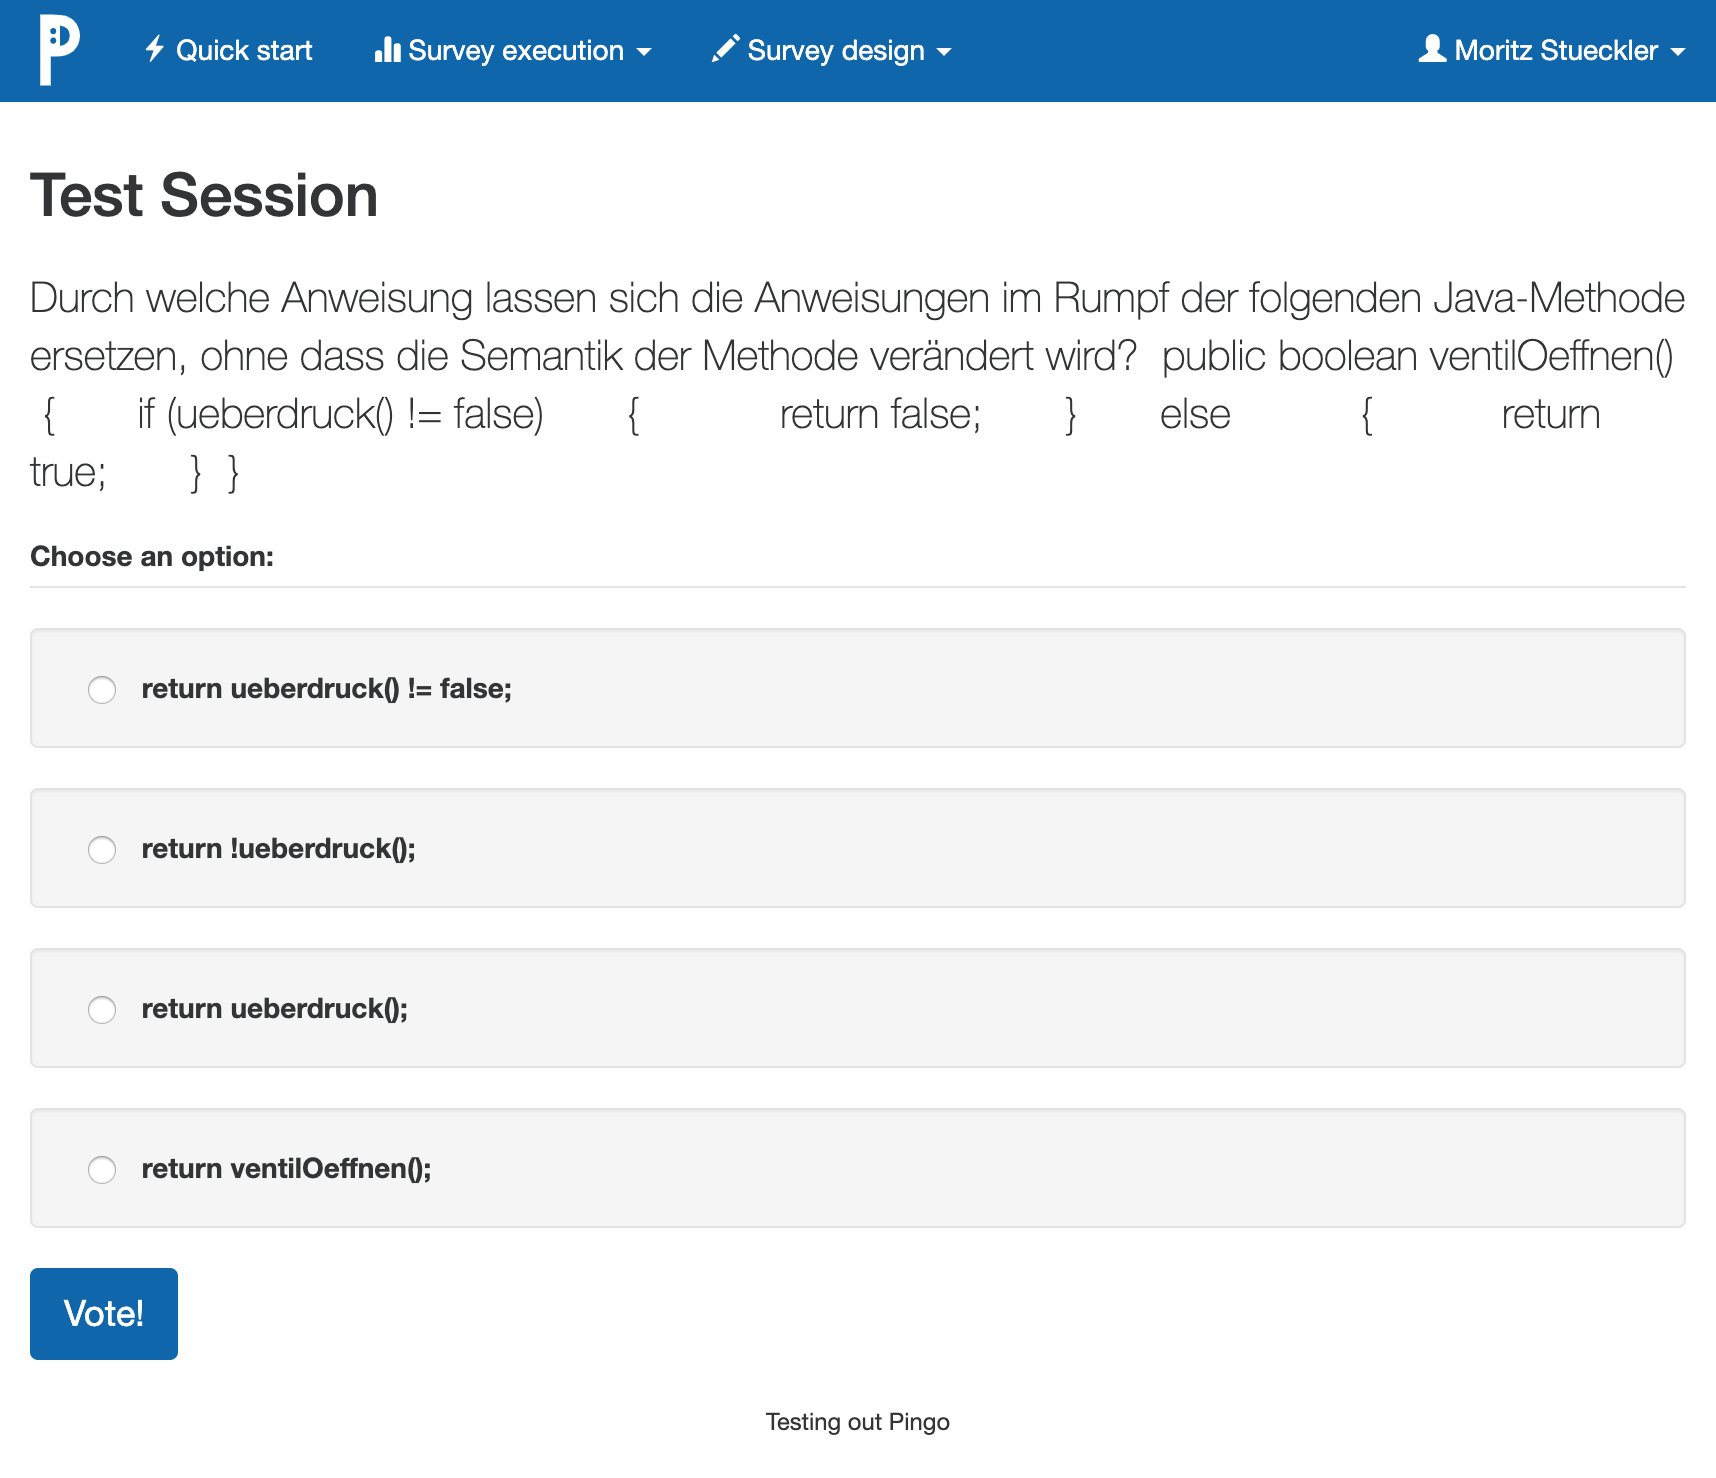
\includegraphics[width=12cm]{chapter/bewertung/bilder/pingo_problem1.png}
    \centering
    \caption{Pingo verfügt über keinerlei Text-Formatierungsoptionen und ist daher ungeeignet für die Darstellung von Quelltext.}
    \label{Abbildung 2.4}
\end{figure}
